\chapter{Результаты исследования}

\begin{figure}
	\begin{center}
		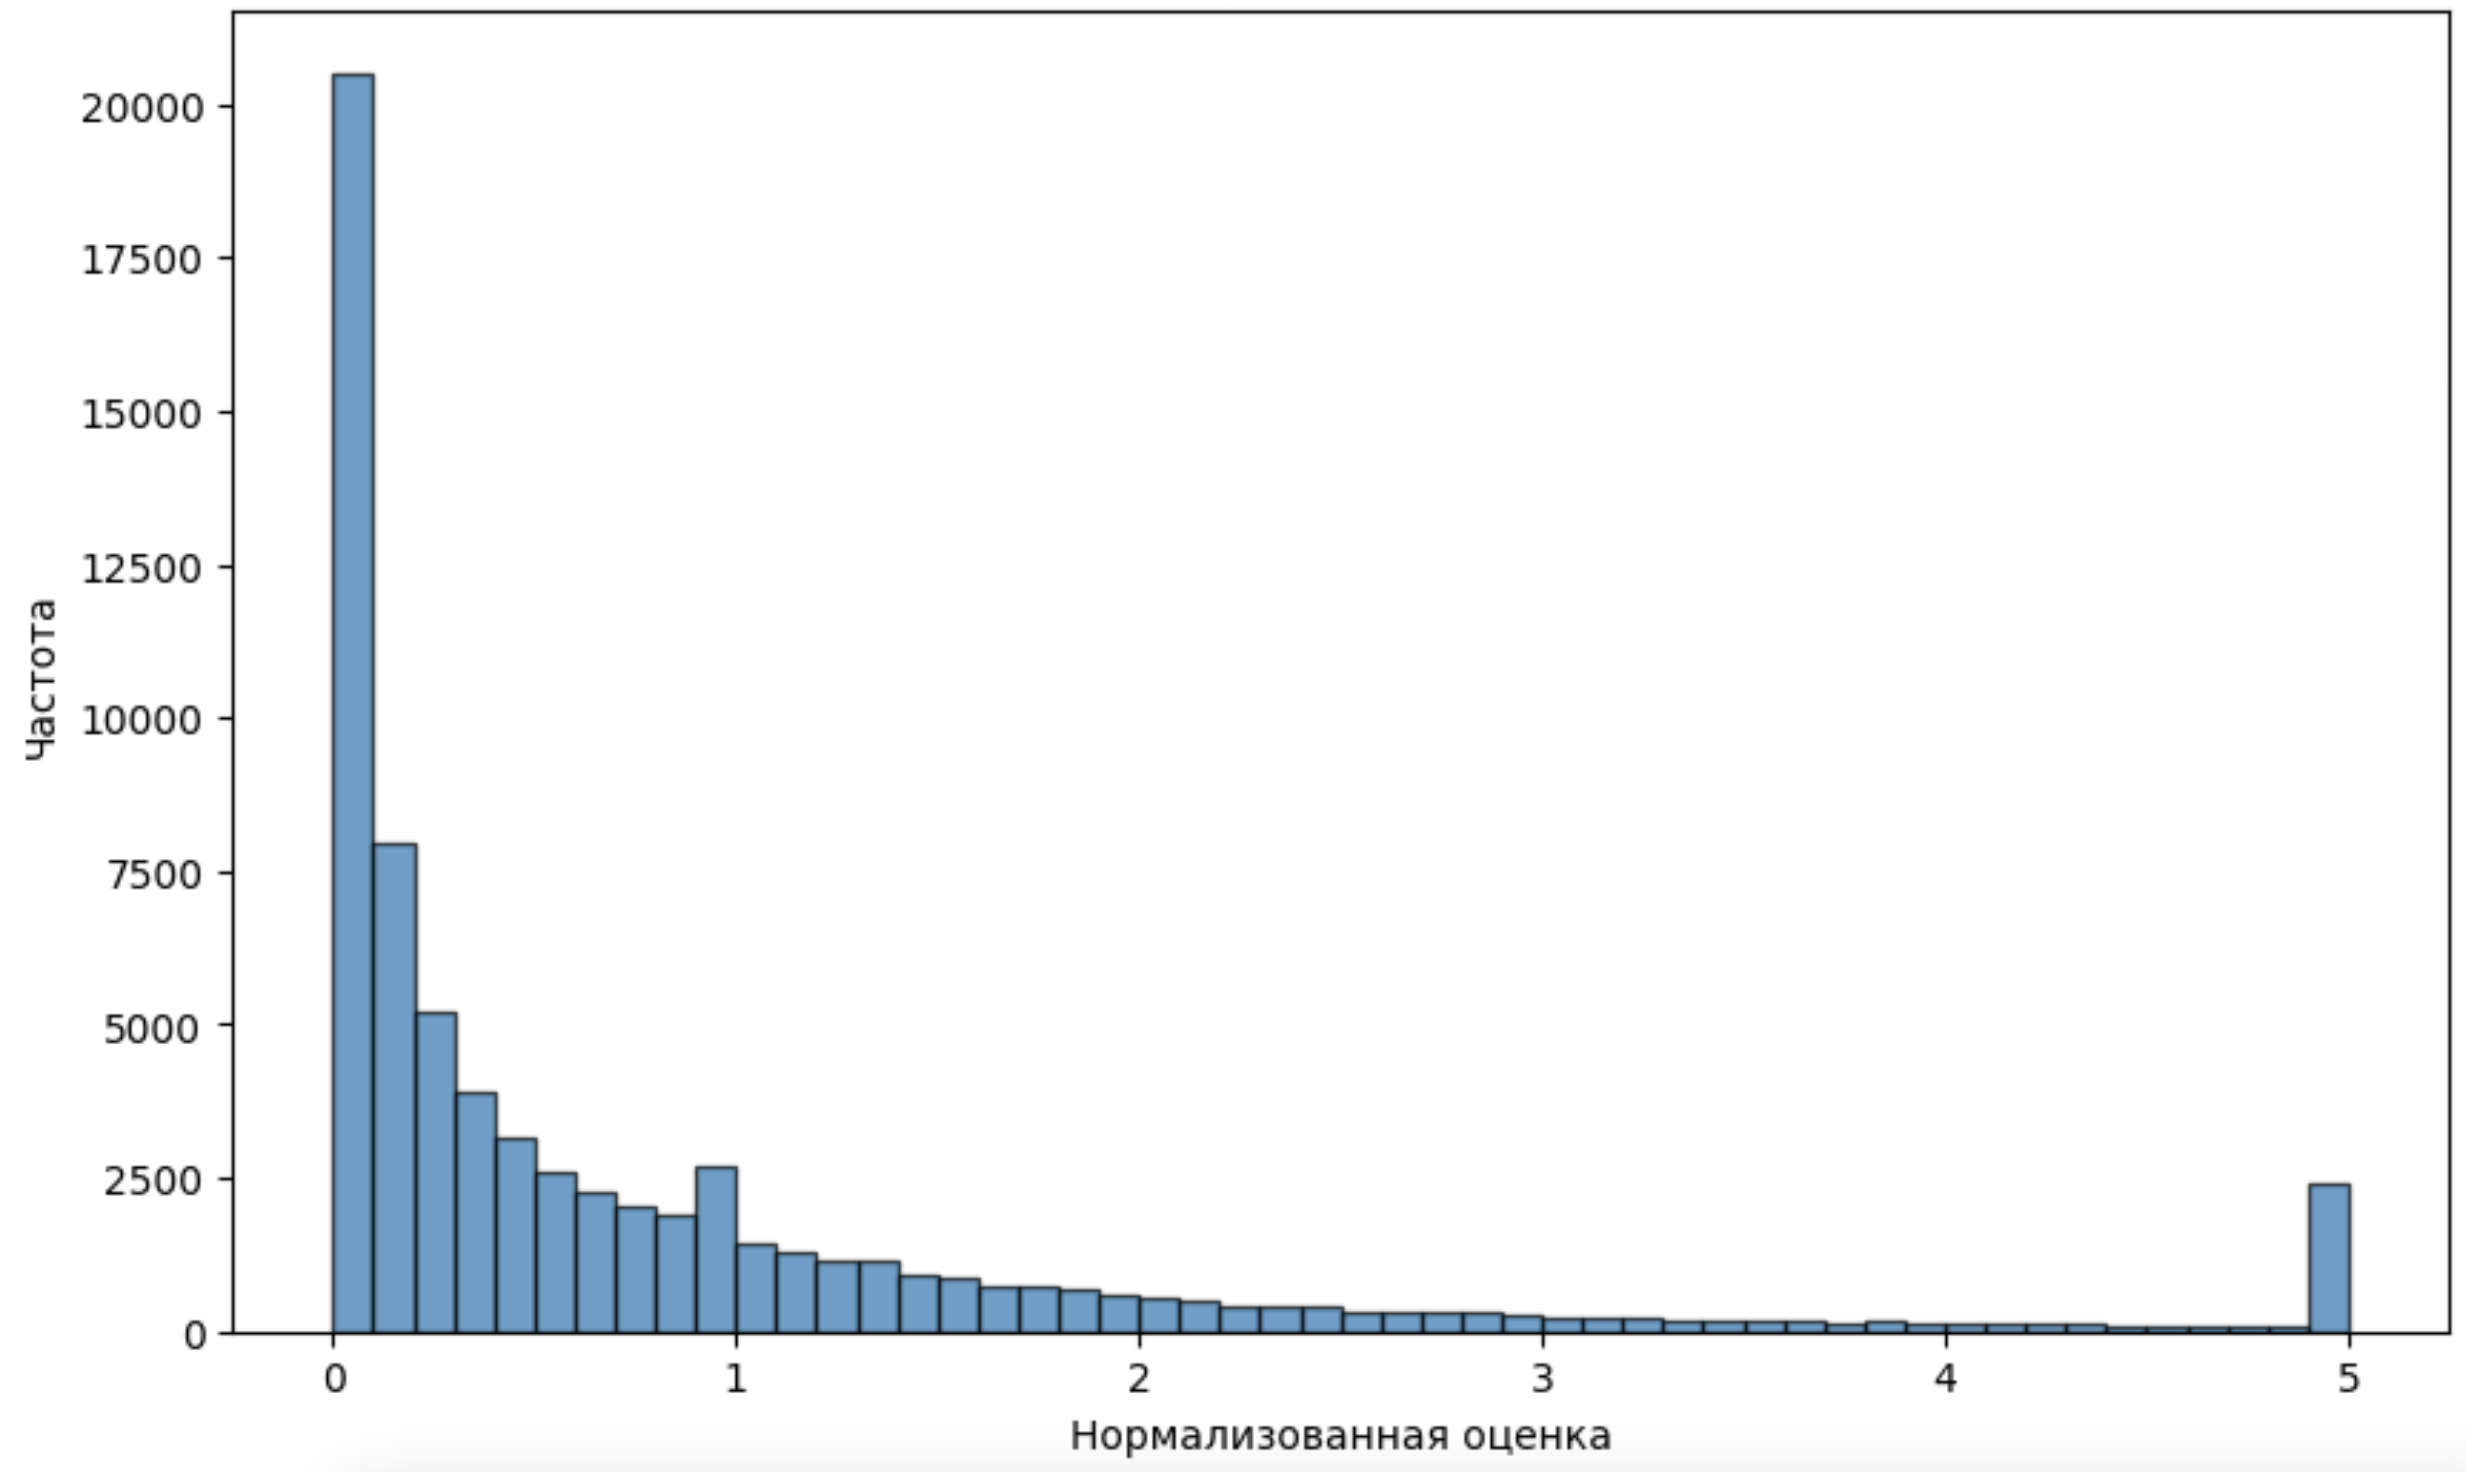
\includegraphics[width=\textwidth]{images/1.png}
	\end{center}
	\caption{Распределение нормализованных оценок пользователей}
	\label{img:1}
\end{figure}

\begin{figure}
	\begin{center}
		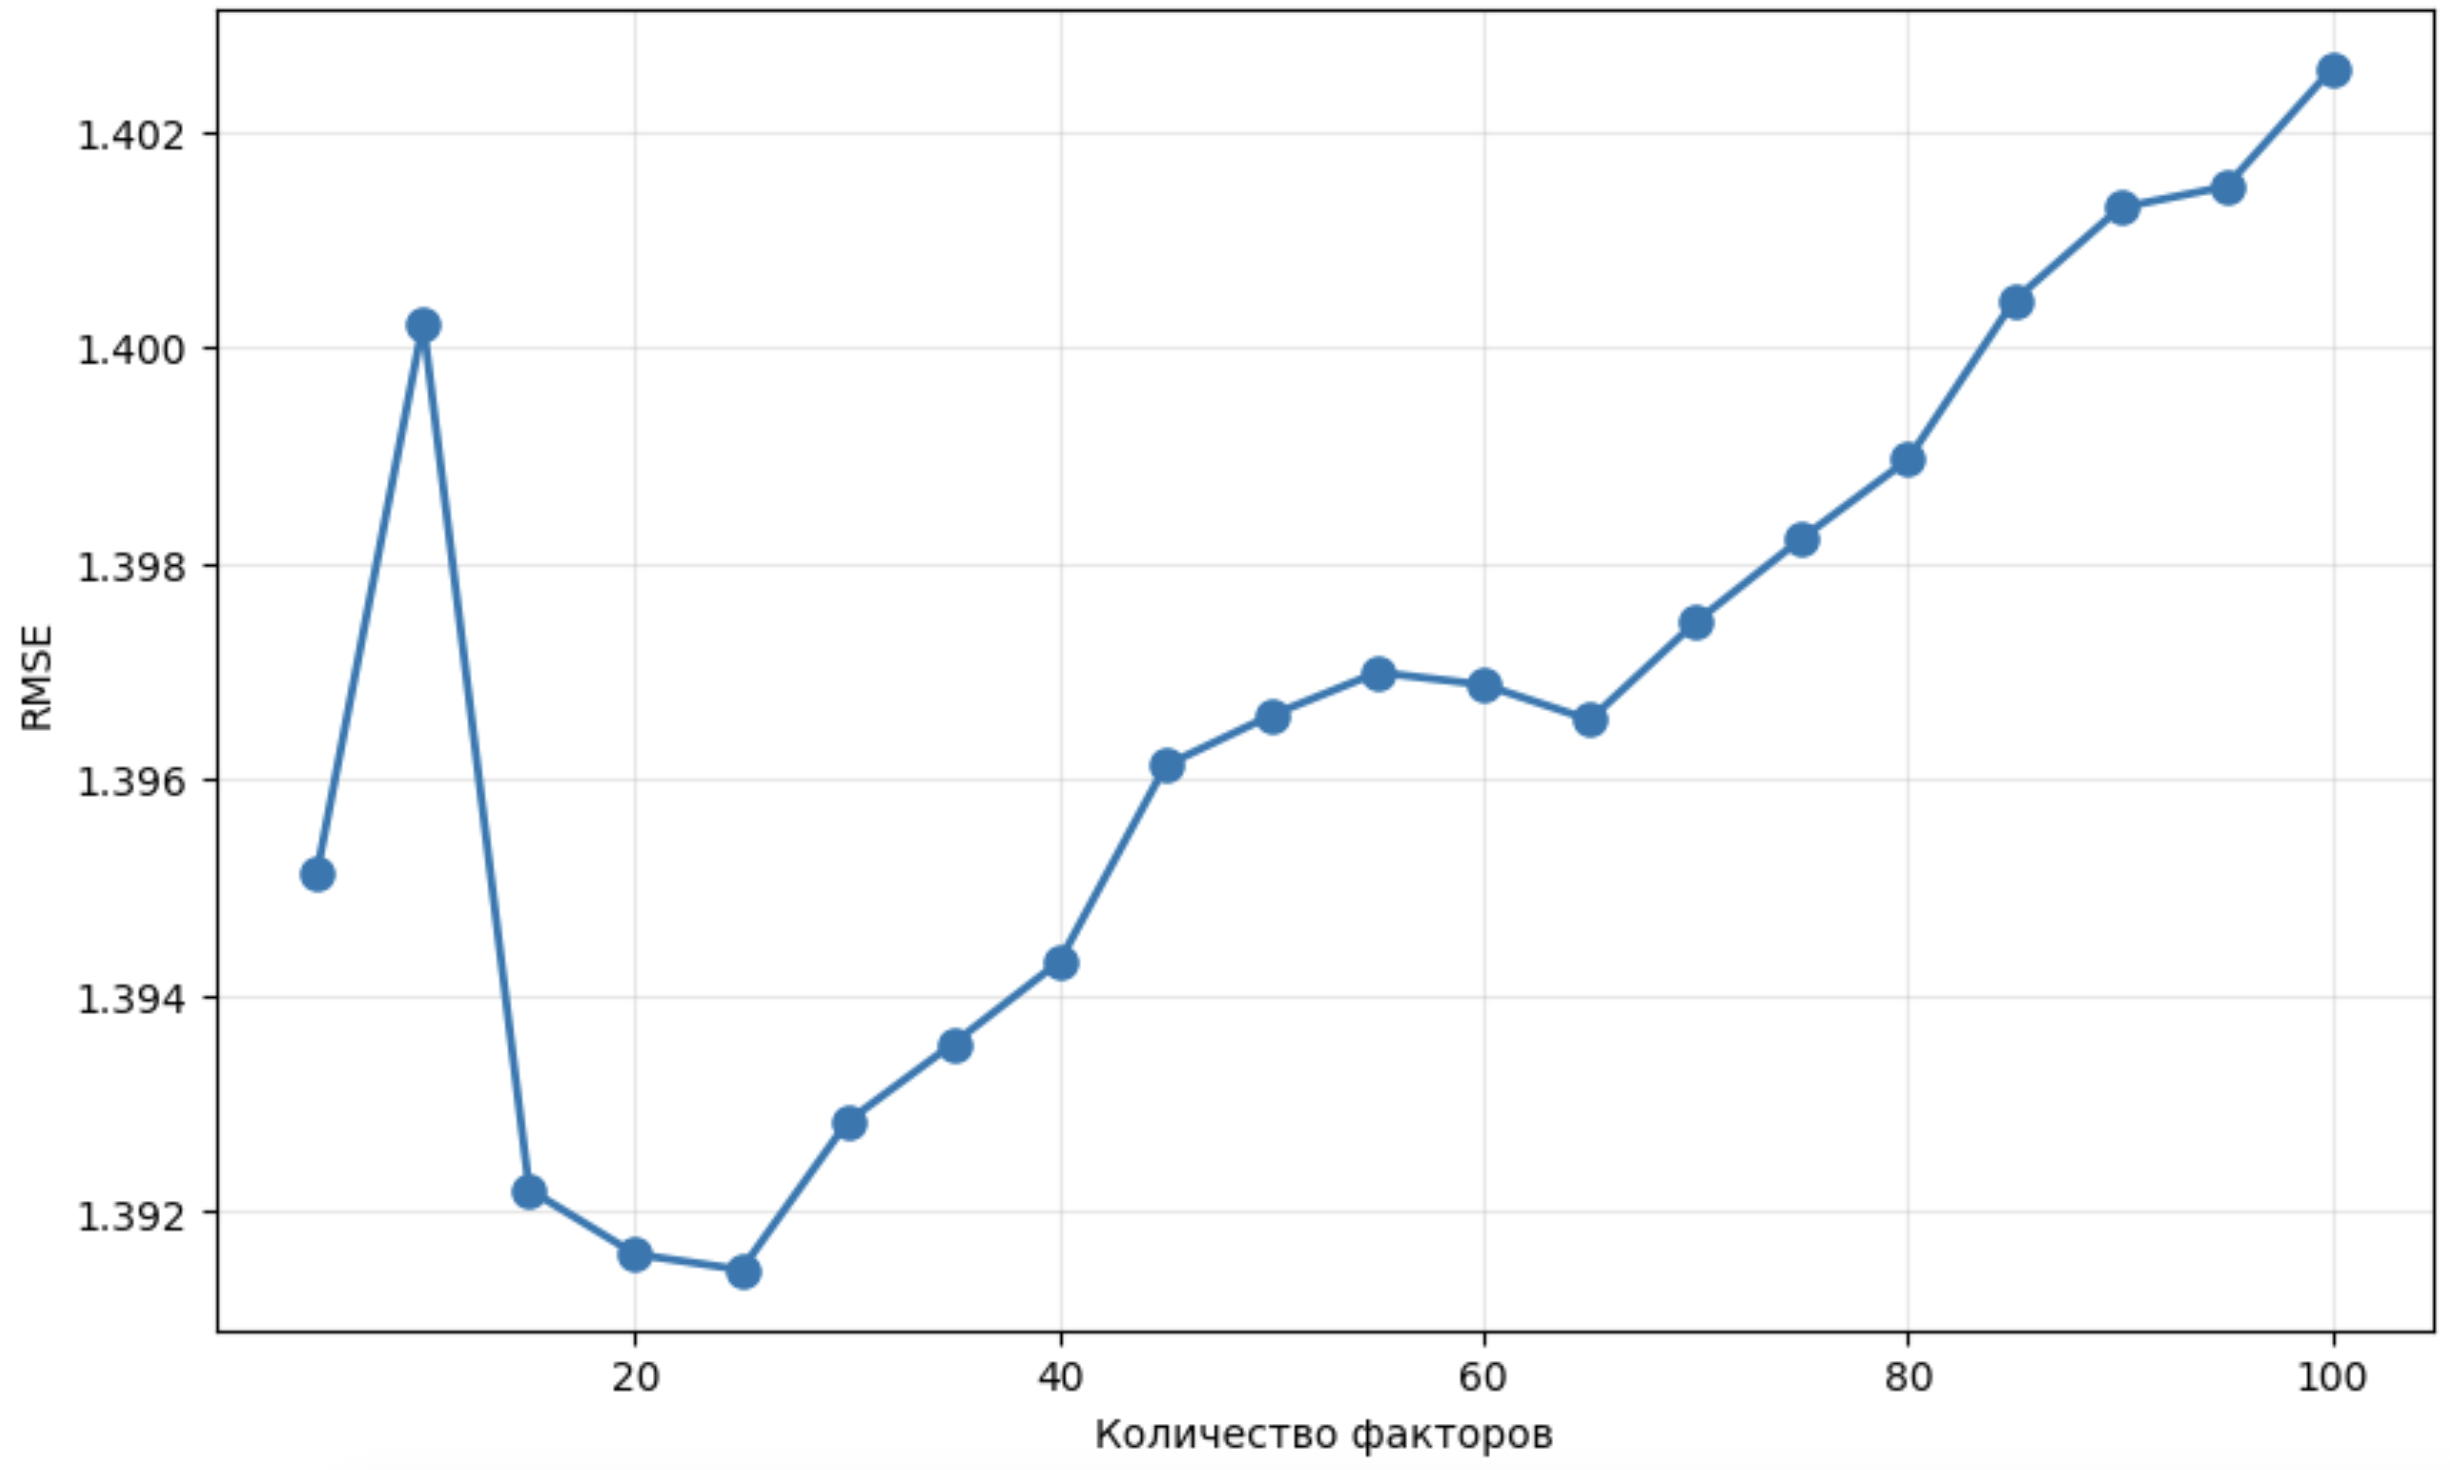
\includegraphics[width=\textwidth]{images/2.png}
	\end{center}
	\caption{Зависимость значения ошибки RMSE от количества компонент SVD при использовании матричной факторизации}
	\label{img:2}
\end{figure}

\begin{figure}
	\begin{center}
		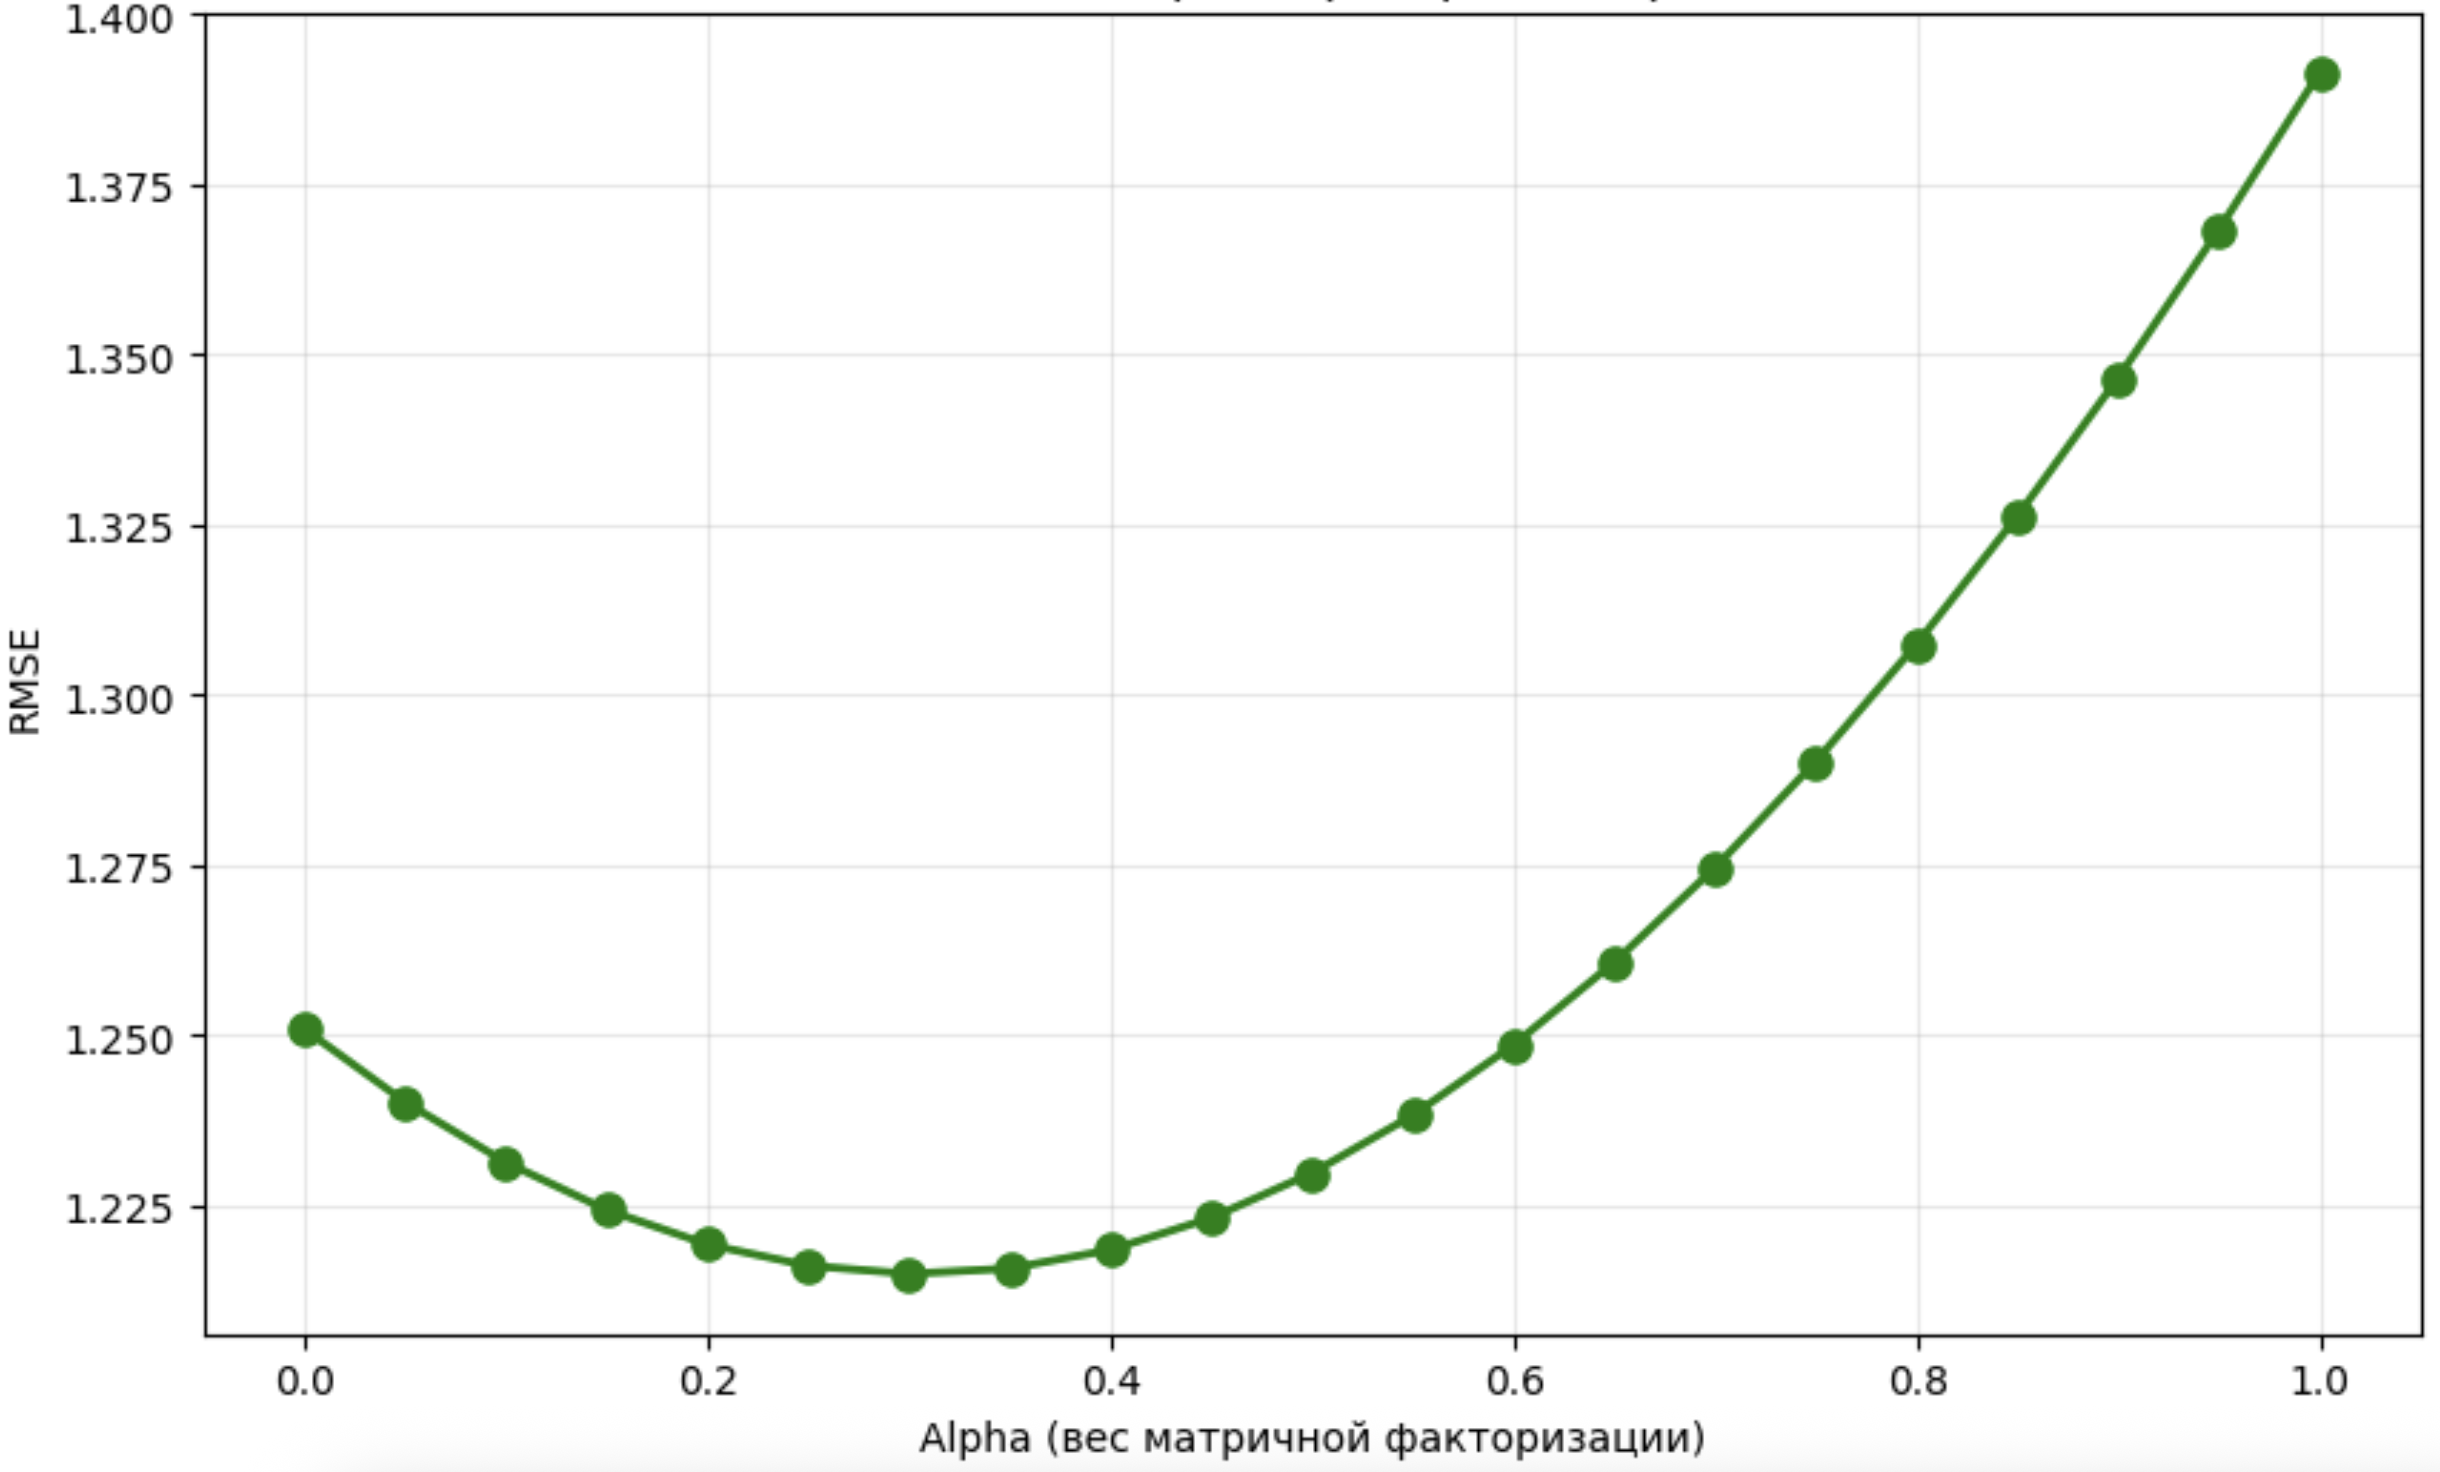
\includegraphics[width=\textwidth]{images/3.png}
	\end{center}
	\caption{Зависимость значения ошибки RMSE от параметра смешивания оценок в гибридной системе}
	\label{img:3}
\end{figure}

\begin{figure}
	\begin{center}
		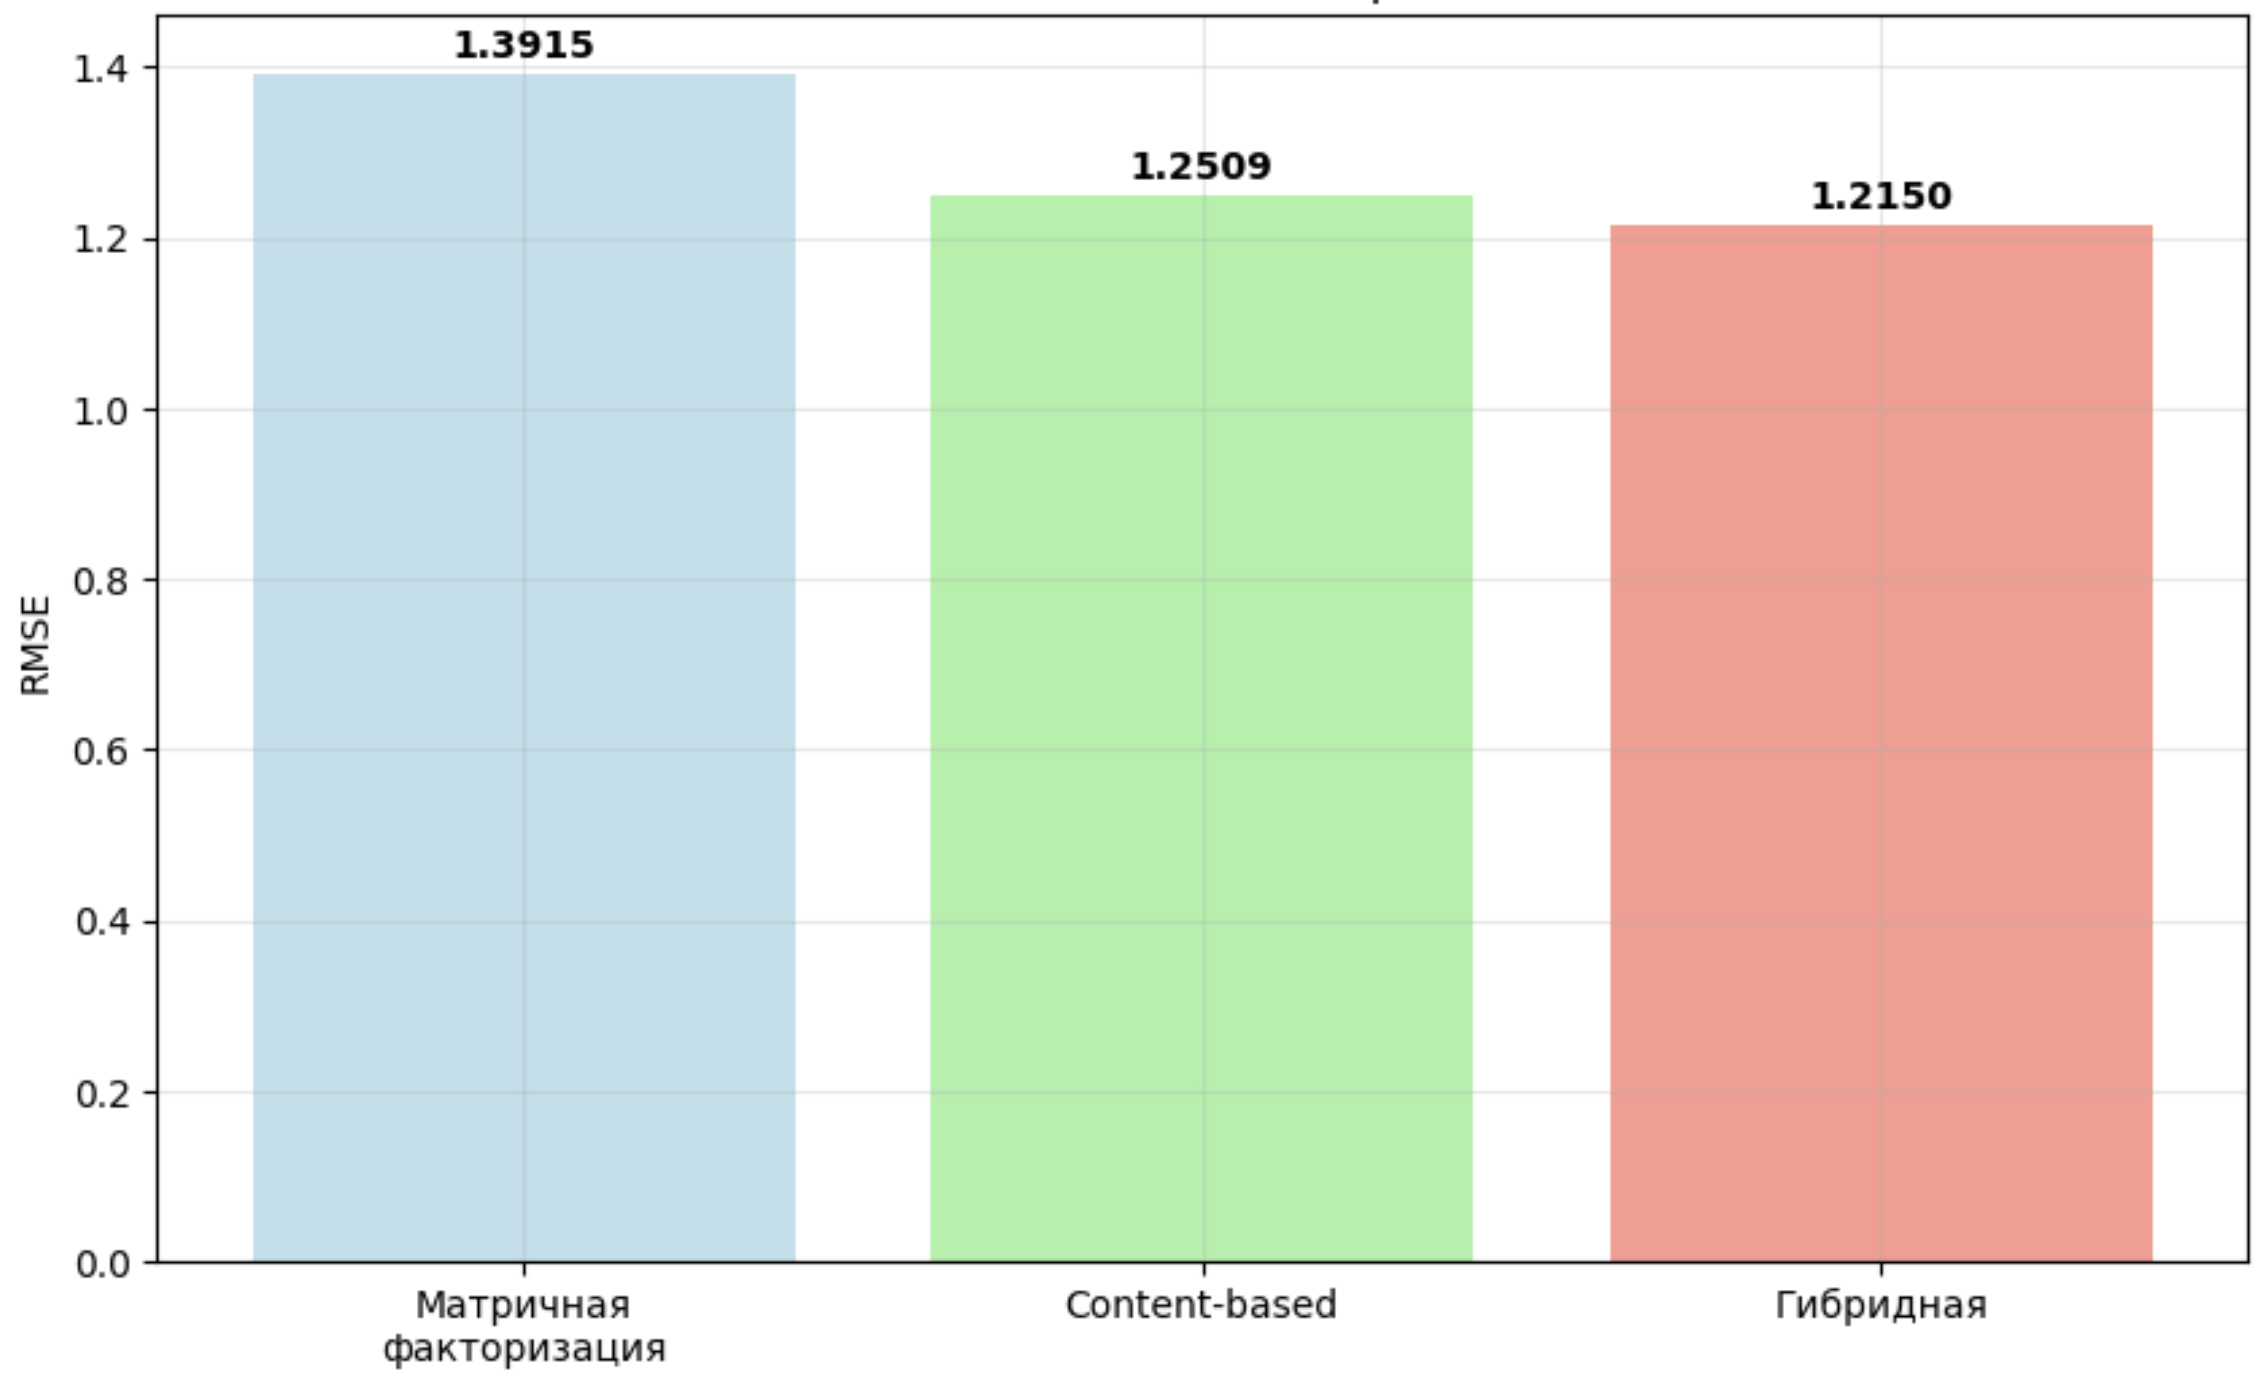
\includegraphics[width=\textwidth]{images/4.png}
	\end{center}
	\caption{Минимальные значения ошибки RMSE, достигнутые гибридной системой и каждым алгоритмом в отдельности}
	\label{img:4}
\end{figure}

Минимальное значение ошибки RMSE (1.2150) было достигнуто при использовании параметра гибридизации $\alpha = 0.3$ (доля оценок, полученных с помощью матричной факторизации). Примеры рекомендаций обученной системы приведены в листинге \ref{lst:1}.

\begin{lstlisting}[label=lst:1,caption=Примеры рекомендаций для пользователей]
	@ПОЛЬЗОВАТЕЛЬ@ 60557056
	
	@ТОП-10 ОЦЕНЕННЫХ ИГР@:
	1. Counter-Strike Source
	2. D.I.P.R.I.P. Warm Up
	3. Eternal Silence
	
	@РЕКОМЕНДАЦИИ ГИБРИДНОЙ СИСТЕМЫ@:
	1. Counter-Strike Condition Zero
	2. Steel Ocean
	3. Battle Nations
	4. Sam & Max 301 The Penal Zone
	5. Trove
	
	@РЕКОМЕНДАЦИИ СИСТЕМЫ НА ОСНОВЕ МАТРИЧНОЙ ФАКТОРИЗАЦИИ@:
	1. Half-Life 2 Lost Coast
	2. Half-Life 2 Deathmatch
	3. Alien Swarm
	4. Killing Floor
	5. Counter-Strike Condition Zero

	@РЕКОМЕНДАЦИИ СИСТЕМЫ ФИЛЬТРАЦИИ НА ОСНОВЕ КОНТЕНТА@:
	1. Aerena
	2. Age of Mythology Extended Edition
	3. A Valley Without Wind
	4. A.V.A - Alliance of Valiant Arms
	5. iBomber Defense
\end{lstlisting}

\clearpage
